\documentclass[10pt,a4paper]{article}
\usepackage[utf8]{inputenc}
\usepackage[T1]{fontenc}
\IfFileExists{lmodern.sty}{\usepackage{lmodern}}{}
\usepackage[margin=2cm]{geometry}
\usepackage{amsmath,amssymb,bm,booktabs,xcolor,enumitem,tikz}
\usetikzlibrary{positioning,arrows.meta}
\usepackage[most]{tcolorbox}
\usepackage[hidelinks]{hyperref}
\setlist{itemsep=1pt,topsep=2pt,leftmargin=*}
\newcommand{\vect}[1]{\bm{#1}}
\newtcolorbox{qbox}[1][Questions]{colback=orange!8,colframe=orange!75!black,fonttitle=\bfseries,title={#1},
  left=4pt,right=4pt,top=2pt,bottom=2pt}
\newtcolorbox{kbox}[1]{colback=blue!5,colframe=blue!60!black,fonttitle=\bfseries,title={#1},
  left=4pt,right=4pt,top=2pt,bottom=2pt}

\begin{document}
\begin{center}
{\Large\bfseries Draft: Mamba for 3D Gaussian Splatting, and Improving Mamba in 4D}\\[2pt]
Muhammad Hussain Qureshi (MSDS25010) \quad·\quad Advisor: Dr.\ Ali Murtaza \quad·\quad 12 November 2026
\end{center}

\begin{kbox}{Summary}
\begin{itemize}
\item \textbf{3D:} treat the Gaussians of a volume as a \emph{point cloud} and process them with Mamba, following
PointMamba~\cite{pointmamba}: order the Gaussians along a space-filling (Hilbert) curve, run Mamba over that
sequence, and let it predict corrections to every Gaussian. Neighbouring Gaussians are then coupled, which acts as a
learned spatial prior when measurements are scarce. Fitted per volume with the physics loss, as now.
\item \textbf{4D:} the current Mamba scans only over \emph{time}, each Gaussian on its own. The main improvement is to
add the same PointMamba-style \emph{spatial} scan, so that Gaussians that move together (one vortex) share
information; plus a faster parallel scan, a tuned smoothness weight and more flows.
\item One shared module (``Gaussian Mamba'') serves both: scan over space in 3D, over space and time in 4D.
\end{itemize}
\end{kbox}

\section{Background}
\textbf{PointMamba}~\cite{pointmamba} (NeurIPS 2024) applies Mamba to point clouds. Key points are chosen by
farthest-point sampling; each key point and its $k$ nearest neighbours form a patch, embedded by a small PointNet
into a token. Because Mamba is a 1D sequence model, the tokens are \emph{serialised} along two space-filling
curves (Hilbert and Trans-Hilbert), so that neighbours in the sequence are neighbours in space. A learned
\emph{order indicator} (scale and shift per ordering) tells the two sequences apart; they are concatenated and processed
by a plain stack of Mamba blocks. It is pre-trained by masked point modelling.
\textbf{Gamba}~\cite{gamba} uses Mamba blocks with learnable 3D Gaussian tokens to predict Gaussian parameters from a
single image, trained on Objaverse. \textbf{Our 4D model} already uses Mamba as the deformation network, scanning
each Gaussian's trajectory over 21 time steps.

\textbf{Difference from those works.} They learn from large datasets of images or shapes. Our problem is a
\emph{per-volume} inverse problem: a few hundred to a few thousand complex measurements from the physics operator,
no camera images and, in 3D, only 30 real volumes. So the Mamba network must work as a \emph{prior inside the
per-volume fit}, like our 4D deformation network, rather than as a pre-trained feed-forward predictor (that is a
Thesis II option, Section~\ref{sec:learned}).

\section{Proposed 3D method: PointMamba over Gaussians}
\begin{center}
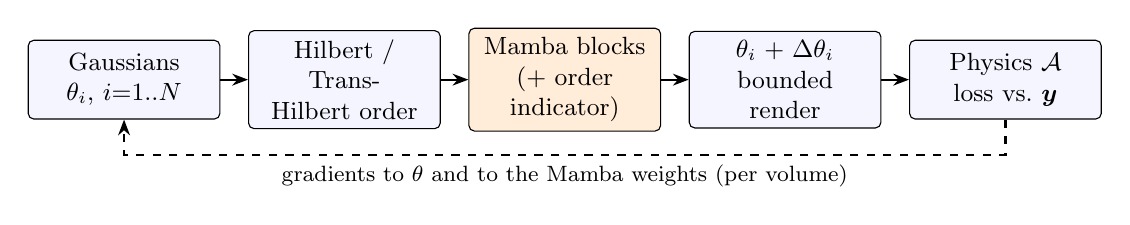
\begin{tikzpicture}[box/.style={draw,rounded corners=2pt,align=center,font=\small,fill=blue!4,minimum height=1cm,text width=2.2cm},
 hl/.style={box,fill=orange!15}, arr/.style={-{Stealth[length=2mm]},thick}, node distance=0.35cm]
\node[box] (g) {Gaussians\\$\theta_i$, $i{=}1..N$};
\node[box,right=of g] (s) {Hilbert /\\Trans-Hilbert order};
\node[hl,right=of s] (m) {Mamba blocks\\(+ order indicator)};
\node[box,right=of m] (d) {$\theta_i+\Delta\theta_i$\\bounded render};
\node[box,right=of d] (a) {Physics $\mathcal{A}$\\loss vs.\ $\vect{y}$};
\draw[arr] (g)--(s); \draw[arr] (s)--(m); \draw[arr] (m)--(d); \draw[arr] (d)--(a);
\draw[arr,dashed] (a.south) -- ++(0,-0.45) -| node[pos=0.25,below,font=\footnotesize]{gradients to $\theta$ and to the Mamba weights (per volume)} (g.south);
\end{tikzpicture}
\end{center}

\begin{enumerate}
\item \textbf{Tokens.} Each Gaussian is one token (no patches needed: Gaussians are already local primitives;
$N\approx$ 4--6k). Token features: Fourier features of the centre $\vect\mu_i$, the current parameters
$\theta_i$ (scales, rotation, amplitude), and optionally the back-projected residual
$\operatorname{Re}\mathcal{A}^H(\vect y-\mathcal{A}f)$ sampled at $\vect\mu_i$, i.e.\ what the measurements still
ask for at that location (``physics-aware token'').
\item \textbf{Serialisation.} Quantise the centres to the grid and sort them by Hilbert index and by Trans-Hilbert
index (axes permuted). Re-sort after every densify / prune step. Order indicator as in PointMamba.
\item \textbf{Network.} 2--4 Mamba blocks ($d=64$, state 16), both orderings, outputs scattered back to Gaussian
order and averaged. The head predicts $\Delta\theta_i$ (amplitude, scales, rotation, small position offset) and is
\textbf{initialised to zero}, so training starts exactly from the current best method (bounded, grid-initialised
Gaussians) and Mamba can only add.
\item \textbf{Fitting.} $\min_{\theta,\phi}\ \lVert\mathcal{A}\tilde f_{\theta+\Delta_\phi(\theta)}-\vect y\rVert^2/\lVert\vect y\rVert^2+\lambda\,\overline{\tilde f}$
with the bounded density $\tilde f=1-e^{-f}$, same sparsity, densification and Adam as now.
\item \textbf{Why it may help.} Without Mamba every Gaussian is optimised on its own; the only coupling is through
the operator. Along the Hilbert sequence Mamba shares information between neighbours (a learned smoothness /
shape prior, similar in spirit to Deep Image Prior). We expect the gain where data are scarcest (60 receivers,
true 3D).
\end{enumerate}

\paragraph{Experiments (true 3D BBBC024 + synthetic; 2D cells with a 2D Hilbert curve).}
\begin{center}
\begin{tabular}{ll}
\toprule
Variant & Tests \\
\midrule
B+G (current best, no network) & baseline \\
Per-Gaussian MLP (same head, no sequence) & is it the network or the coupling? \\
Mamba, random order & does spatial order matter? \\
Mamba, Hilbert & PointMamba serialisation \\
Mamba, Hilbert + Trans-Hilbert + order indicator & full PointMamba design \\
\quad + residual token features & physics-aware tokens \\
Voxel grid (same loss) & reference \\
\bottomrule
\end{tabular}
\end{center}
360 / 180 / 60 receivers, 3 volumes (5 if time allows); PSNR, SSIM, parameters, time. About one Kaggle run (6--8\,h).

\paragraph{Later option (Thesis II): learned PointMamba reconstructor.}\label{sec:learned}
Train one PointMamba network across many volumes (synthetic nuclei plus BBBC024, train/test split) to map the
physics-aware Gaussian tokens to parameter updates, unrolled for a few steps (a learned optimiser), optionally
pre-trained by PointMamba's masked modelling on Gaussian sets fitted to volumes. Faster at test time and a stronger
prior, but needs a training set and much more compute.

\section{Improving Mamba in 4D}
Current result: with 10\% observations and temporal smoothness, Mamba beats the MLP by 2.4\,dB on unseen frames;
with full observations they tie, and Mamba is about 9$\times$ slower. Limits of the current design: each Gaussian's
trajectory is processed \emph{independently} (no interaction between Gaussians), the sequence has only 21 steps, the
scan is a sequential Python loop, and the smoothness weight was not tuned.
\begin{enumerate}
\item \textbf{Space--time Mamba (main idea).} Alternate the existing temporal scan (per Gaussian, over $t$) with a
PointMamba spatial scan (per frame, over Gaussians in Hilbert order), as in factorised video Mamba models. A vortex
is many Gaussians moving together; the spatial scan lets them share motion. Same module as the 3D method.
\item \textbf{Parallel scan.} Replace the sequential loop by a chunked parallel (log-space cumulative) scan, or the
official CUDA kernel if it installs on Kaggle: expected 5--10$\times$ faster, needed anyway for the spatial scan
over thousands of Gaussians.
\item \textbf{Velocity-based deformation.} Predict a velocity per Gaussian and time step and integrate it
($\vect\mu_i(t+1)=\vect\mu_i(t)+\vect v_i(t)\Delta t$) instead of an independent offset per frame: physically
consistent motion, natural for a recurrent model.
\item \textbf{Tuning and statistics.} Sweep the smoothness weight ($\lambda_T\in\{0.1,0.3,1,3\}$), the number of
Gaussians, and evaluate 5--10 flows instead of 3 (possible once the scan is fast).
\item \textbf{Optional physics.} Penalise the vorticity-equation residual
$\partial_t\omega+\vect u\cdot\nabla\omega-\nu\Delta\omega-f$ on the rendered frames (spectral derivatives). You said
4D is fine for now, so this stays optional.
\end{enumerate}

\section{Plan}
\begin{tabular}{ll}
\toprule
Step & Time \\
\midrule
Shared Gaussian-Mamba module, Hilbert serialisation, parallel scan; unit tests & 1--2 days \\
3D: PointMamba-over-Gaussians variants (table above), Kaggle run & 1 day + 8\,h GPU \\
4D: space--time Mamba, velocity deformation, $\lambda_T$ sweep, more flows, Kaggle run & 1 day + 8\,h GPU \\
Results into thesis, slides and poster & 1--2 days \\
\bottomrule
\end{tabular}

\begin{qbox}[To confirm with Dr.\ Murtaza]
\begin{enumerate}
\item Is ``PointMamba over the Gaussians, fitted per volume'' what you meant, or a pre-trained network across
volumes (Section~\ref{sec:learned})?
\item Should Mamba be compared only with the current Gaussians and the voxel grid, or also with a Transformer over
the same tokens?
\end{enumerate}
\end{qbox}

\begin{thebibliography}{9}\small
\bibitem{pointmamba} D.~Liang, X.~Zhou, W.~Xu, X.~Zhu, Z.~Zou, X.~Ye, X.~Tan, X.~Bai. PointMamba: A Simple State Space
Model for Point Cloud Analysis. NeurIPS 2024. arXiv:2402.10739.
\bibitem{gamba} Q.~Shen, Z.~Wu, X.~Yi, P.~Zhou, H.~Zhang, S.~Yan, X.~Wang. Gamba: Marry Gaussian Splatting with Mamba
for Single-View 3D Reconstruction. arXiv:2403.18795, 2024.
\bibitem{mamba} A.~Gu, T.~Dao. Mamba: Linear-Time Sequence Modeling with Selective State Spaces. arXiv:2312.00752, 2023.
\end{thebibliography}
\end{document}
